\chapter{Fonctionnement des cryptomonnaies}
\label{ch:presentation}

\section{Qu'est-ce qu'une cryptomonnaie ?}

Dans un premier temps, il est nécessaire de comprendre comment fonctionne une cryptomonnaie avant de pouvoir en créer une. Et il faut tout d'abord pouvoir définir \emph{qu'est-ce qu'une cryptomonnaie}.

Une cryptomonnaie est un ensemble de mécanismes cryptographiques utilisés dans le but de sécuriser un registre distribué afin d'obtenir un système de paiement décentralisé. Plus simplement, une cryptomonnaie est un système de paiement qui n'est pas régit par une entité centrale, comme une banque par exemple, et qui permet à tout le monde d'émettre des transactions qui seront incluses dans un registre. Ce registre est publique et partagé avec tous les utilisateurs via un réseau pair-à-pair. Le plus souvent, ce registre est représenté sous forme de chaîne de blocs, chaque bloc contenant ou un certain nombre de transactions. C'est la \emph{blockchain}. 

Mais comme partout, il y a des personnes hônnetes mais aussi des gens malhônnetes qui vont essayer d'abuser des failles du système. Dans le cas d'un système de paiement décentralisé, il n'y a pas de banque pour vérifier la validité des transactions ce qui pose un réel problème de sécurité. Du coup, pour rendre le système sûr, on utilise de la cryptographie. La cryptographie, grâce à des preuves mathématiques, rend la validité (ou non) des transactions quasiement irréfutable et permet à n'importe qui de vérifier les transactions stockées dans la blockchain.

Chaque utilisateur possède une copie de cette blockchain sur son ordinateurs et peut recevoir de nouvelles transactions d'autres utilisateurs et en envoyer lui-même. Voyons maintenant comment fonctionne plus en détails une blockchain avec un exemple compréhensible dans la section suivante.

\section{La blockchain}

Comme vu ci-dessus, une cryptomonnaie est en fait un simple registre numérique dans lequel chacun peut ajouter des transactions. Imaginons maintenant un exemple simple avec les utilisateurs Alice, Bob et Charlie. Chacun d'entre eux peut ajouter une ligne au registre qui dit par exemple << Alice paie Bob 5 CHF >>, << Bob paie Charlie 8 CHF >>. Et, à interval régulier, ils se regroupent pour se transmettre l'argent qu'ils ont indiqué dans le registre.

\begin{figure}[H]
  \centering
  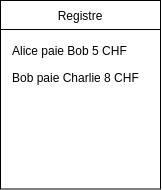
\includegraphics[width=4cm]{images/crypto_1.png}
  \caption{Exemple de registre de transactions simplifié}
\end{figure}

Seulement rien n'empêche Bob de rajouter la première ligne << Alice paie Bob 5 CHF >> autant de fois qu'il veut sans le consentement d'Alice.

\begin{figure}[H]
  \centering
  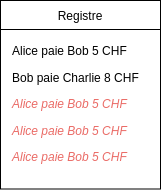
\includegraphics[width=4cm]{images/crypto_2.png}
  \caption{Bob inscrit de fausses transactions dans le registre}
\end{figure}

C'est là que la cryptographie rentre en jeu. Plus précisément les \glspl{signature}. Chaque transaction va être accompagnée d'une signature. Les signatures numériques reposent sur de la \gls{crypto_asym}. C'est à dire que chaque utilisateur possède une pair de clé : une clé publique $pk$ et une clé privée (ou secrète) $sk$. La clé publique de chaque personne est partagée avec tous les autres utilisateurs du registre alors que la clé privée reste bien cachée chez son propriétaire et n'est jamais divulguée à qui que ce soit.

À la différence des signatures manuscrites sur papier qui sont à chaque fois presque identiques, une signature numérique change en fonction du message à signer. Pour signer ce message, on utilise la clé privée. On peut alors imaginer la signature d'un message $m$ avec la fonction suivante :

\begin{equation*}
  \mathsf{Sign(m, sk)} = \mathsf{signature}
\end{equation*}

Pour vérifier une signature numérique, on utilise la clé publique associée à la clé privée utilisée pour signer le message. Comme cette clé est connue de tous, tout le monde peut vérifier la signature du message :

\begin{equation*}
  \mathsf{Verify(m, signature, pk)} = \{\mathsf{Vrai}, \mathsf{Faux}\}
\end{equation*}

Ainsi, au lieu de simplement ajouter une transaction au registre, les utilisateurs devront préalablement signer leur transaction et inscrire cette signature à coté de la transaction dans le registre. Cela permet de prouver que l'émetteur de la transaction est consentent. Les autres utilisateurs peuvent vérifier la signature de la transaction émise grâce à la clé publique de l'émetteur. Si la signature est correct, ils peuvent être quasiment certains que c'est bien l'émetteur de la transaction qui l'a signée car il est extrêmement difficile de forger une signature valide quand on ne possède pas la clé privée. Par exemple, si Alice souhaite inscrire une nouvelle transaction dans le registre, elle le ferait de la manière suivante :

\begin{align*}
  \mathsf{transaction_{Alice}} &= \textsf{"Alice paie Bob 5 CHF"}\\
  \mathsf{signature} &= \mathsf{Sign(transaction_{Alice}, sk_{Alice})}
\end{align*}

\begin{figure}[H]
  \centering
  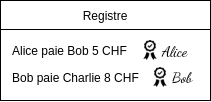
\includegraphics[width=6cm]{images/crypto_3.png}
  \caption{Les transations du registre sont maintenant signées numériquement}
\end{figure}

De cette manière, Bob ne peut plus rajouter de lignes sans le consentement d'Alice car il ne possède par sa clé privée. A noté également que lors de la vérification de la signature, la clé publique doit appartenir à la personne qui envoie de l'argent, sinon la transaction est rejetée. Cela fait sens car Bob peut signer << Alice paie Bob 10 CHF >> et la signature sera techniquement valide mais le contenu du message n'est pas juste. Bob ne peut pas demander de l'argent dans le registre. C'est uniquement la personne qui signe la transaction qui donne de l'argent. 

Cependant, même si Bob ne connaît pas la clé privée d'Alice, il peut quand même ré-envoyer une ancienne transaction signée par Alice. Sa signature sera toujours valide.

\begin{figure}[H]
  \centering
  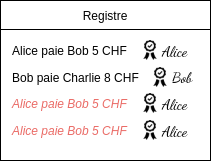
\includegraphics[width=6cm]{images/crypto_4.png}
  \caption{Bob inscrit deux anciennes transactions d'Alice}
\end{figure}

C'est pour cela qu'on inclut un identifiant unique, comme un nombre, à la transaction afin d'obtenir une signature différente à chaque transation même si elles sont identiques. Cela force Alice à refaire une signature à chaque nouvelle transaction et empêche Bob de réutiliser une ancienne signature valide d'Alice.

\begin{figure}[H]
  \centering
  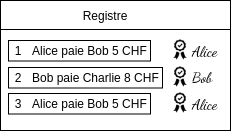
\includegraphics[width=6cm]{images/crypto_5.png}
  \caption{Un identifiant unique est signé avec la transaction}
\end{figure}

Maintenant, imaginons qu'un des utilisateurs, Charlie par exemple, doive beaucoup d'argent et ne vienne pas au rendez-vous pour payer les autres utilisateurs. Il peut écrire autant de transaction qu'il veut dans le registre et rien ne l'empêche de ne pas venir pour payer les autres. Il faut alors trouver un moyen où les utilisateurs n'ont pas besoin de se retrouver pour payer se qu'ils doivent.

On peut imaginer un système dans lequel les utilisateurs mettent une certaine somme d'argent dans un panier commun au début, disons 100 CHF et les premières lignes du registre indiquerait combien ils ont mis.

\begin{figure}[H]
  \centering
  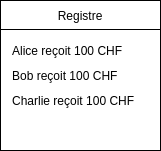
\includegraphics[width=4cm]{images/crypto_6.png}
  \caption{Premières lignes indiquant la somme initiale donnée par chaque utilisateur}
\end{figure}

Comme cela, on peut empêcher les utilisateurs de faire des transactions dont le montant dépasse ce qu'il possède dans le registre. Par exemple, si Charlie paie à Alice et Bob 50 CHF chacun, il ne pourra plus payer 10 CHF à nouveau à Bob car son solde est trop faible.

\begin{figure}[H]
  \centering
  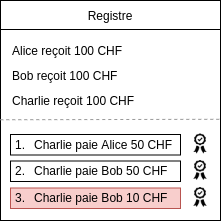
\includegraphics[width=5.5cm]{images/crypto_7.png}
  \caption{Charlie n'as pas assez d'argent pour effectuer la troisième transaction}
\end{figure}

Cela implique de conserver l'historique complet des transactions pour pouvoir donner le montant restant d'un utilisateur.

Avec ce système, on a une très bonne séparation entre l'argent dans le registre et l'argent réel. On peut même utiliser une monnaie propre au registre, par exemple des << jetons >>. Les utilisateurs sont libres d'échanger des jetons contre des francs suisse et inversément, cependant le taux de change entre les deux va dépendre de l'offre et de la demande puisqu'il y a un nombre limité de \emph{jetons} dans le registre. Par exemple, Alice peut donner à Bob 20 CHF et Bob, en échange, écrit une transaction dans le registre de 20 \emph{jetons} pour Alice.

Vient maintenant un autre problème avec ce registre. Qui est-ce qui gère le registre ? Qui est-ce qui vérifie si les transactions écrites sont valides ? Cela peut être une personne déléguée à cette tâche. C'est ce qui se fait souvent avec les cryptomonnaies privées car il est possible de désigner quelqu'un de confiance pour gèrer le registre. Cependant, un des objectif de Satoshi Nakamoto lors qu'il a écrit son document sur le Bitcoin est de faire un système de paiement décentralisé. Un système dans lequel il n'y a pas d'entité centrale qui gère ce fameux registre. Ce qu'il propose est alors très simple: chaque utilisateur possède sa propre copie du registre. Comme ça c'est décentralisé et quand une personne souhaite effecuter une transaction, il l'envoie à tous les autres pour qu'ils l'ajoutent à leur registre. Mais on peut se demander: << Comment est-on sûr que tout le monde possède la même version du registre ? >>. Effectivement, si Bob envoie une transaction à Alice mais pas à Charlie, ils n'auront alors plus la même version du registre et par conscéquant ne pourront plus calculer correctement leur solde lorsqu'ils voudront faire une nouvelle transaction. Du coup la question est : << À quelle version du register peut-on faire confiance ? >>.

Pour palier à ce problème, dans son papier, Satoshi Nakamoto explique qu'il faut avoir confiance dans le registre qui possède le plus de travail de calcul. Le travail de calcul (\emph{computational work} en anglais) utilise des \glspl{hash-function}. Une fonction de hachage prend des données en entrée et donne une empreinte numérique en sortie. Cette empreinte semble complétement aléatoire mais n'est en réalité pas aléatoire car deux mêmes entrées donneront toujours la même empreinte. Une autre propriété importante des fonctions de hachage est le fait il est impossible de retrouver les données d'entrée à partie de l'empreinte. Il n'y a pas de meilleure méthode que de tester toutes les données possibles en entrée jusqu'à obtenir l'empreinte souhaitée. Et c'est sûr cette propriété que ce base l'algorithme de preuve de travail.

Le consensus par preuve de travail fonctionne de la manière suivante : on commence par découper le registre en blocs. Chaque bloc peut contenir un certain nombre de transactions. On assemble les données d'un bloc avec un nombre choisi et on passe le tout dans une fonction de hachage. On recalcul l'empreinte de ces données en modifiant le nombre jusqu'à que cette dernière commence par un nombre défini de \emph{zéros}. Plus l'empreinte commence par un nombre important de zéros plus le travail de calcul est grand. En effet, avec par exemple avec 30 << 0 >> au début de l'empreinte, en considérant un message aléatoire, la probabilité de trouver un hash commençant par 30 zéros est de $\frac{1}{2^{30}}$ soit 1 chance sur 1073741824. Ce-dessous une illustration d'une preuve de travail :

\begin{figure}[H]
  \centering
  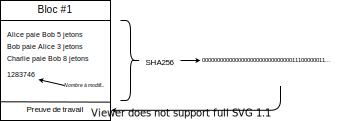
\includegraphics[width=\textwidth]{images/crypto_8}
  \caption{Calcul de la preuve de travail d'un bloc}
\end{figure}

Comme cela, un bloc n'est valide que lorsqu'il possède une preuve de travail correct, au même titre qu'une transaction n'est valide que lorsqu'elle est signée par l'envoyeur.

Pour créer une suite dans les blocs, on va inclure dans l'en-tête du bloc l'empreinte du bloc précédent. Ainsi, si on modifie les données d'un ancien bloc, cela changera son empreinte et il sera nécessaire de recalculer sa preuve de travail et celle de tous les bloc qui suivent.

\begin{figure}[H]
  \centering
  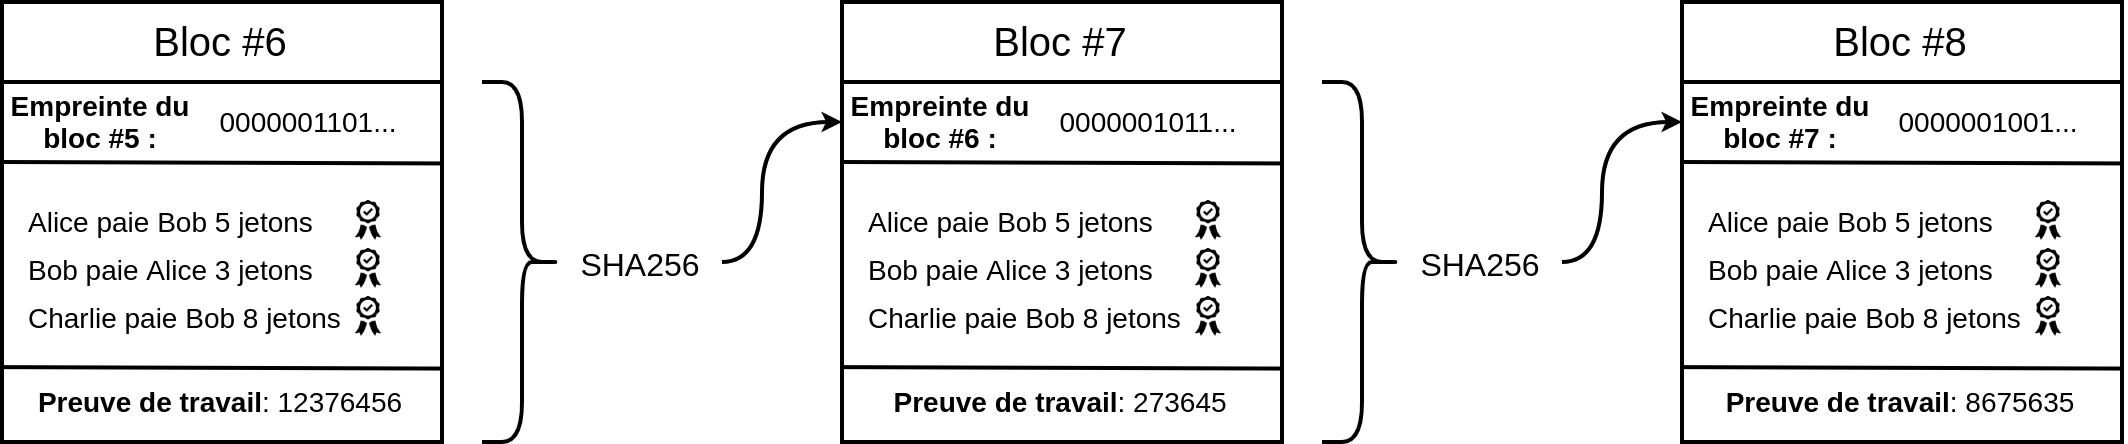
\includegraphics[width=\textwidth]{images/crypto_9}
  \caption{Calcul de la preuve de travail d'un bloc}
\end{figure}

On a maintenant une chaîne de blocs, une << blockchain >>. Les utilisateurs vont, chacun de leur côté, essayer de faire un bloc en trouvant la preuve de travail associée. Le premier qui trouve une preuve de travail va publier le bloc. Les autres utilisateurs vont alors se baser sur ce nouveau bloc pour tenter de trouver la preuve de travail et publier leur bloc. C'est en quelques sortes une course à qui trouvera la preuve en premier et comme le travail de calcul dépend de la puissance de calcul des ordinateurs, les plus puissants auront plus de chance de la trouver en premier. 

Pour répondre à la question: << Comment être sûr que tout le monde à le même registre ? >>, il suffit de conserver la chaîne qui a le plus de travail de calcul. Dans la majorité des cas c'est la chaîne de blocs contenant le plus de blocs. Cela car en cas de fraude, l'attaquant devra être capable de trouver les preuves de travail tous seul plus rapidement que tous les autres utilisateurs. Par exemple, si Bob envoie un bloc avec des transactions de sa part à Alice mais ne l'envoie pas à Charlie, Alice aura une version franduleuse de la chaîne. Pour qu'Alice continue à croire que c'est la bonne chaîne, Bob doit être capable de trouver la preuve de travail des nouveaux blocs avant Alice et Charlie. Chose qui est difficile à faire car Bob ne possède qu'un ordinateur pour le calcul alors qu'Alice et Charlie ont chacun un ordinateur. Bob a du coup moins de puissance de calcul que les autres ce qui veut dire qu'Alice et Charlie, à eux deux, arriveront à terme à trouver des preuves plus rapidement que Bob. La chaîne frauduleuse de Bob ne sera alors plus la plus longue et Alice arrêtera de faire confiance à cette branche de la chaîne. Grâce à ce principe de preuve de travail, il est nécessaire de possèder plus de 50\% de la puissance de calcul total des utilisateurs pour pouvoir émettre une chaîne frauduleuse. C'est l'attaque des 51 pourcents. Ce principe a d'ailleur été utilisé bien avant l'apparition des blockchains pour sécuriser les messageries contre les spams.

Nous avons vu ici l'illustration d'une blockchain simplifée fonctionnant plus ou moins de la même manière que le Bitcoin avec quelques simplification. Avec Bitcoin, le nombre de zéros est défini par le réseau pour maintenir un temps de création de bloc d'environ 10 minutes. En effet, si on demande plus de zero au début de l'empreinte, cela prendra plus de temps à calculer et inversement si on souhaite moins de zéros. Le réseau adapte alors ce nombre en fonction de la puissance disponible. Si des utilisateurs partent, il y aura moins de puissance de calcul disponible, le réseau diminuera alors le nombre de zeros et inversement si des utilisateurs se joigne au réseau.

On peut remarquer qu'une grande partie de la sécurité de la décentralisation repose sur le protocole de consensus et sur le fait que tous les utilisateurs sont d'accord sur la même version de blockchain. L'algorithme de consensus est en effet le coeur d'une blockchain et il en exite plein de différent, la preuve de travail (proof of work) étant le plus connu. C'est pour cela qu'un étude plus approfondie sur les protocoles de consensus est réalisée sur dans le chapitre suivant.
